\section{连续性方程}
在\xref{sec:非平衡载流子的寿命}的\xref{eq:非平衡载流子的寿命方程},曾讨论过均匀光注入下$\delt{p}$随时间的衰减,得到了非平衡载流子的寿命
\begin{Equation}
    \dv{\delt{p}}{t}=-\frac{\delt{p}}{\tau}
\end{Equation}
在\xref{sec:载流子的扩散运动}的\xref{eq:稳态扩散下的方程},曾讨论过稳态扩散,即非均匀光注入下$\delt{p}$随空间的衰减
\begin{Equation}
    D_\text{p}\dv[2]{\delt{p}}{x}=\frac{\delt{p}}{\tau}
\end{Equation}
这两者分别涉及了非平衡载流子的随时间和空间的变化,但是尚且不够完备。
\begin{itemize}
    \item 仅讨论非平衡载流子$\delt{p}$的分布是比较狭隘的。注入不均和掺杂不均分别会导致平衡载流子$p_0$和非平衡载流子$\delt{p}$的分布不均,较一般的,我们应建立关于$p$的微分方程。
    \item 仅讨论扩散亦是狭隘的。扩散电流和漂移电流是可以同时存在的。
    \item 在一般情况下$p=p(x,t)$同时为空间和时间的函数,换言之$p$需用偏微分方程描述。
\end{itemize}\nopagebreak
在本节,我们的目标是,建立最一般情况下,载流子浓度$p$适用的偏微分方程(连续性方程)。\goodbreak

我们要关注的是,载流子浓度$p$随时间的变化率$\pdv*{p}{t}$由哪些部分构成
\begin{enumerate}
    \item 扩散电流$(J)_\text{扩}$的负通量源(汇),当然需要除以电荷量$q$。
    \item 漂移电流$(J)_\text{漂}$的负通量源(汇),当然需要除以电荷量$q$。
    \item 复合消失的非平衡载流子(单位时间单位体积)。
    \item 其他可能导致载流子浓度变化外界因素。
\end{enumerate}
由此,我们可以建立起连续性方程的基本形态\setpeq{连续性方程}
\begin{Equation}&[1]
    \pdv{p}{t}=-\frac{1}{q}\pdv{(J_\text{p})_\text{扩}}{x}-\frac{1}{q}\pdv{(J_\text{p})_\text{漂}}{x}-\frac{\delt{p}}{\tau}+g_\text{p}
\end{Equation}
根据\fancyref{fml:载流子的漂移扩散}
\begin{Equation}&[2]
    (J_\text{p})_\text{扩}=-qD_\text{p}\pdv{p}{x}\qquad
    (J_\text{p})_\text{漂}=qp\mu_\text{p}\Emf
\end{Equation}
求导得(注意电场$\Emf$也与$x$有关)
\begin{Equation}&[3]
    \pdv{(J_\text{p})_\text{扩}}{x}=-qD_\text{p}\pdv[2]{p}{x}\qquad
    \pdv{(J_\text{p})_\text{漂}}{x}=q\mu_\text{p}\Emf\pdv{p}{x}+q\mu_\text{p}p\pdv{\Emf}{x}
\end{Equation}
将\xrefpeq{3}代入\xrefpeq{1},这就得到了连续性方程的最终形态
\begin{BoxEquation}[连续性方程]
    \uwave{连续性方程}描述了少数载流子浓度的时空分布规律
    \begin{Equation}
        \pdv{p}{t}=D_\text{p}\pdv[2]{p}{x}-\mu_\text{p}\Emf\pdv{p}{x}-\mu_\text{p}p\pdv{\Emf}{x}-\frac{\delt{p}}{\tau}+g_\text{p}
    \end{Equation}
\end{BoxEquation}
现在,让我们在两种特殊情况下,求解连续性方程,两种特殊情况均有一些共通的简化
\begin{enumerate}
    \item 设其他因素$g_\text{p}$为零,即$g_\text{p}=0$。
    \item 设电场是均匀的,有$\pdv*{\Emf}{x}=0$。
    \item 设材料掺杂是均匀的,有$\pdv*{p_0}{x}=0$,或者$\pdv*{p}{x}=\pdv*{\delt{p}}{x}$。
\end{enumerate}
此时我们可以得到\fancyref{eqt:连续性方程}的简化形式,这是关于$\delt{p}$的
\begin{Equation}[简化连续性方程]
    D_\text{p}\pdv[2]{\delt{p}}{x}
    -\mu_\text{p}\Emf\pdv{\delt{p}}{x}
    -\frac{\delt{p}}{\tau}=\pdv{\delt{p}}{t}
\end{Equation}
这里说明一下,之所以$\pdv*{p}{t}=\pdv*{\delt{p}}{t}$,这是因为平衡载流子$p_0$总是非时变的。\footnote{对此存疑,但也未找到更进一步的解释,姑且认同。}

\subsection{光照恒定下的稳态漂移扩散}\setpeq{光照恒定下的稳态漂移扩散}
光照恒定即假定这是稳态扩散,因此$p$非时变,即$\pdv*{p}{t}=0$,这时\xref{eq:简化连续性方程}可以再简化为
\begin{Equation}&[1]
    D_\text{p}\pdv[2]{\delt{p}}{t}-\mu_\text{p}\Emf\pdv{\delt{p}}{t}-\frac{\delt{p}}{\tau}=0
\end{Equation}
关于$\delt{p}(x,t)$的偏微分方程由此简化为了关于$\delt{p}(x)$的常微分方程,它的通解是
\begin{Equation}&[2]
    \delt{p}=A\exp(\lambda_1x)+B\exp(\lambda_2x)
\end{Equation}
这里$\lambda_1,\lambda_2$是特征根方程的解(这是求解二阶线性齐次常微分方程的步骤)
\begin{Equation}&[3]
    D_\text{p}\lambda^2-\mu_\text{p}\Emf\lambda-\frac{1}{\tau}=0
\end{Equation}
两端乘$\tau$
\begin{Equation}&[4]
    \tau D_\text{p}\lambda^2-\tau\mu_\text{p}\Emf\lambda-1=0
\end{Equation}
这里,引入有关漂移的\uwave{牵引长度}和有关漂移的\uwave{扩散长度}(Diffusion Length)作为代换变量\footnote{实际上,扩散长度$L_\text{p}$在\xref{subsec:样品足够厚}时已经被引入过了。}
\begin{BoxDefinition}[牵引长度]
    牵引长度表征了漂移特性,定义为
    \begin{Equation}
        L_\text{p}(\Emf)=\Emf\mu_\text{p}\tau
    \end{Equation}
\end{BoxDefinition}
\begin{BoxDefinition}[扩散长度]
    扩散长度表征了扩散特性,定义为
    \begin{Equation}
        L_\text{p}=\sqrt{D_\text{p}\tau}
    \end{Equation}
\end{BoxDefinition}
特别要注意,$L_\text{p}\neq L_\text{p}(\Emf)$,两者毫无关系!\setpeq{光照恒定下的稳态漂移扩散}

根据\fancyref{def:牵引长度}和\fancyref{def:扩散长度},\xrefpeq{4}可以表示为
\begin{Equation}
    L_\text{p}^2\lambda-L_\text{p}(\Emf)\lambda-1=0
\end{Equation}
解得
\begin{Equation}
    \lambda_1,\lambda_2=\frac{1}{2L_\text{p}^2}\qty[L_\text{p}(\Emf)\pm\sqrt{L_\text{p}^2(\Emf)+4L_\text{p}^2}]
\end{Equation}
显然
\begin{Equation}
    \lambda_1>0\qquad\lambda_2<0
\end{Equation}\goodbreak
由于我们这里的光注入是从半导体的$x=0$一端注入的(边界条件总是要的),因此\xrefpeq{2}的通解中,正指数项$A\exp(\lambda_1 x)$需要被舍去($A=0$),负指数项$B\exp(\lambda_2x)$得到保留
\begin{Equation}
    \delt{p}=B\e^{\lambda_2x}
\end{Equation}
在$x=0$处,有$\delt{p}=(\delt{p})_0$
\begin{Equation}
    \delt{p}=(\delt{p})_0\exp(\lambda_2 x)
\end{Equation}
这里$\lambda_2$是由牵引长度$L_\text{p}(\Emf)$和扩散长度$L_\text{p}$共同确定的,换言之,由漂移和扩散共同确定
\begin{Equation}
    \lambda_2=\frac{1}{2L_\text{p}^2}\qty[L_\text{p}(\Emf)-\sqrt{L_\text{p}^2(\Emf)+4L_\text{p}^2}]
\end{Equation}
但若电场很强或很弱,使漂移和扩散中有一者可以被忽略,那$\lambda_2$将仅由$L_\text{p}$或$L_\text{p}(\Emf)$决定。

\begin{BoxFormula}[电场很强时的稳态漂移扩散]
    若电场很强,扩散可以忽略,此时$\delt{p}$的行为由牵引长度决定
    \begin{Equation}
        \delt{p}=(\delt{p})_0\exp[-\frac{x}{L_\text{p}(\Emf)}]
    \end{Equation}
\end{BoxFormula}
\begin{Proof}
    这是因为,当$L_\text{p}(\Emf)\gg L_\text{p}$时
    \begin{Equation}
        \sqrt{L_\text{p}^2(\Emf)+4L_\text{p}^2}=L_\text{p}(\Emf)\qty[1+\frac{4L_\text{p}^2}{L_\text{p}^2(\Emf)}]^{\frac{1}{2}}\approx L_\text{p}(\Emf)\qty[1+\frac{2L_\text{p}^2}{L_\text{p}^2(\Emf)}]
    \end{Equation}
    因此
    \begin{Equation}*
        \lambda_2=\frac{1}{2L_\text{p}^2}\qty[L_\text{p}(\Emf)-L_\text{p}(\Emf)-\frac{2L_\text{p}^2}{L_\text{p}(\Emf)}]=-\frac{1}{L_\text{p}(\Emf)}\qedhere
    \end{Equation}
\end{Proof}

\begin{BoxFormula}[电场很弱时的稳态漂移扩散]
    若电场很弱,漂移可以忽略,此时$\delt{p}$的行为由扩散长度决定
    \begin{Equation}
        \delt{p}=(\delt{p})_0\exp[-\frac{x}{L_\text{p}}]
    \end{Equation}
\end{BoxFormula}
\begin{Proof}
    这是因为,当$L_\text{p}(\Emf)\ll L_\text{p}$时
    \begin{Equation}
        \sqrt{L_\text{p}^2(\Emf)+4L_\text{p}^2}\approx 2L_\text{p}
    \end{Equation}
    因此
    \begin{Equation}*
        \lambda_2=\frac{1}{2L_\text{p}^2}\qty[L_\text{p}(\Emf)-2L_\text{p}]=\frac{1}{2L_\text{p}^2}\qty[-2L_\text{p}]=-\frac{1}{L_\text{p}}\qedhere
    \end{Equation}
\end{Proof}
实际上,\xref{fml:电场很弱时的稳态漂移扩散}就是先前\xref{sec:载流子的扩散运动}中,讨论样品足够厚时的扩散运动时得到的\xref{fml:样品足够厚时非平衡载流子的浓度分布}。\goodbreak

\subsection{光脉冲下的漂移扩散}
光脉冲即假定在初始时刻,光注入的非平衡载流子$\delt{p}$的分布局限在$x=0$附近一个很窄的范围内,换言之,非平衡载流子的浓度$\delt{p}(x,t)$具有狄拉克函数的初值条件\setpeq{光脉冲下的漂移扩散}
\begin{Equation}&[1]
    \delt{p}(x,0)=N_\text{p}\dirac(x)
\end{Equation}
光脉冲条件下,$\delt{p}$满足的方程就是\xrefeq{简化连续性方程},没什么再可简化的了
\begin{Equation}&[2]
    D_\text{p}\pdv[2]{\delt{p}}{x}
    -\mu_\text{p}\Emf\pdv{\delt{p}}{x}
    -\frac{\delt{p}}{\tau}=\pdv{\delt{p}}{t}
\end{Equation}
但简单起见,我们不妨先考虑无外电场,即$\Emf=0$时的情形
\begin{Equation}&[3]
    D_\text{p}\pdv[2]{\delt{p}}{x}-\frac{\delt{p}}{\tau}=\pdv{\delt{p}}{t}
\end{Equation}
假设这个方程的解具有以下形式(目的是将方程的非齐次项$\delt{p}/\tau$消除)
\begin{Equation}&[4]
    \delt{p}(x,t)=f(x,t)\e^{-t/\tau}
\end{Equation}
将它代入\xrefpeq{3}中
\begin{Equation}&[5]
    \qquad\qquad\qquad
    D_\text{p}\pdv[2]{f(x,t)}{x}\e^{-t/\tau}-\frac{1}{\tau}f(x,t)\e^{-t/\tau}=\pdv{f(x,t)}{t}\e^{-t/\tau}-\frac{1}{\tau}f(x,t)\e^{-t/\tau}
    \qquad\qquad\qquad
\end{Equation}
即
\begin{Equation}&[6]
   \pdv{f(x,t)}{t}-D_\text{p}\pdv[2]{f(x,t)}{x}=0
\end{Equation}
这是一个标准的一维无界区域上的热传导方程,根据数学物理,它的解是
\begin{Equation}&[7]
    f(x,t)=\frac{1}{\sqrt{4\pi D_\text{p}t}}\Int[-\infty][\infty]f(\xi,0)\exp[-\frac{(x-\xi)^2}{4D_\text{p}t}]\dd{\xi}
\end{Equation}
而$f(x,0)$是容易求得的,由于$\e^{-t/\tau}$在$t=0$时为$1$
\begin{Equation}&[8]
    f(x,0)=\delt{p}(x,0)=N_\text{p}\dirac(x)
\end{Equation}
将\xrefpeq{8}代入\xrefpeq{7},应用狄拉克函数的筛选性质
\begin{Equation}&[9]
    \qquad\quad
    f(x,t)=\frac{1}{\sqrt{4\pi D_\text{p}t}}\Int[-\infty][\infty]N_\text{p}\dirac(\xi)\exp[-\frac{(x-\xi)^2}{4D_\text{p}t}]\dd{\xi}=\frac{N_\text{p}}{\sqrt{4\pi D_\text{p}t}}\exp[-\frac{x^2}{4D_\text{p}t}]
    \qquad\quad
\end{Equation}
将\xrefpeq{9}代回\xrefpeq{4}
\begin{Equation}&[10]
    \delt{p(x,t)}=f(x,t)\e^{-t/\tau}=\frac{N_\text{p}}{\sqrt{4\pi D_\text{p}t}}\exp[-\frac{x^2}{4D_\text{p}t}-\frac{t}{\tau}]
\end{Equation}
这表明没有外加电场时,光脉冲停止后,非平衡载流子由注入点向两侧以高斯波包的形式扩散,峰值减小,宽度增大。并且,非平衡载流子在扩散过程中还不断发生复合,总量也在减少。\goodbreak

现在,让我们重新来考虑存在电场$\Emf$的一般情况,方程是\xrefpeq{2}
\begin{Equation}&[11]
    D_\text{p}\pdv[2]{\delt{p}}{x}
    -\mu_\text{p}\Emf\pdv{\delt{p}}{x}
    -\frac{\delt{p}}{\tau}=\pdv{\delt{p}}{t}
\end{Equation}
这里的求解非常有技巧性,关键在于作以下变量代换
\begin{Equation}&[12]
    x'=x-\mu_\text{p}\Emf t
\end{Equation}
并相应假设方程的解具有以下形式
\begin{Equation}&[13]
    \delt{p}(x,t)=f(x',t)\e^{-t/\tau}
\end{Equation}
\xrefpeq{11}的左端的代换比较简单,考虑到$\pdv*{x'}{x}=1$
\begin{Equation}&[14]
    \qquad
    D_\text{p}\pdv[2]{\delt{p}}{x}
    -\mu_\text{p}\Emf\pdv{\delt{p}}{x}
    -\frac{\delt{p}}{\tau}=
    D_\text{p}\pdv[2]{f(x',t)}{{x'}}\e^{-t/\tau}-\mu_\text{p}\Emf\pdv{f(x',t)}{x'}\e^{-t/\tau}-\frac{1}{\tau}f(x',t)\e^{-t/\tau}
    \qquad
\end{Equation}
\xrefpeq{11}的右端的代换则复杂些
\begin{Equation}&[15]
    \pdv{\delt{p}}{t}=\pdv{t}\qty[f(x',t)\e^{-t/\tau}]=\pdv{f(x',t)}{t}\e^{-t/\tau}-\frac{1}{\tau}f(x',t)\e^{-t/\tau}
\end{Equation}
这里的麻烦在于$f(x',t)$中的$x'$也与$t$有关,因此
\begin{Equation}&[16]
    \pdv{\delt{p}}{t}=\qty[\pdv{f(x',t)}{x'}\pdv{x'}{t}+\pdv{f(x',t)}{t}]\e^{-t/\tau}-\frac{1}{\tau}f(x',t)\e^{-t/\tau}
\end{Equation}
这里符号有一定歧义
\begin{itemize}
    \item \xrefpeq{15}中的$\pdv*{f(x',t)}{t}$对$t$的偏导是将$x'$也视作$t$的函数。
    \item \xrefpeq{16}中的$\pdv*{f(x',t)}{t}$对$t$的偏导则是将$x'$视作无关常数。
\end{itemize}
类似歧义问题曾在微积分2中充分讨论过。

根据\xrefpeq{12},$\pdv*{x'}{t}=-\mu_\text{p}\Emf$,因此\xrefpeq{16}可以再表示为
\begin{Equation}&[17]
    \pdv{\delt{p}}{t}=\qty[\pdv{f(x',t)}{t}-\mu_\text{p}\Emf\pdv{f(x',t)}{x'}]\e^{-t/\tau}-\frac{1}{\tau}f(x',t)\e^{-t/\tau}
\end{Equation}
展开
\begin{Equation}&[18]
    \pdv{\delt{p}}{t}=\pdv{f(x',t)}{t}\e^{-t/\tau}-\mu_\text{p}\Emf\pdv{f(x',t)}{x'}\e^{-t/\tau}-\frac{1}{\tau}f(x',t)\e^{-t/\tau}
\end{Equation}
比较\xrefpeq{14}和\xrefpeq{18},注意到许多项是可以约掉的,故\xrefpeq{11}可以转化为
\begin{Equation}&[19]
    \pdv{f(x',t)}{t}-D_\text{p}\pdv[2]{f(x',t)}{{x'}}=0
\end{Equation}
注意到\xrefpeq{19}和\xrefpeq{6}的数学形式完全一致,只是$f(x,t)$变为了$f(x',t)$,故
\begin{Equation}
    \delt{p(x,t)}=f(x',t)\e^{-t/\tau}=\frac{N_\text{p}}{\sqrt{4\pi D_\text{p}t}}\exp\qty\Bigg[-\frac{{x'}^2}{4D_\text{p}t}-\frac{t}{\tau}]
\end{Equation}
而代入\xrefpeq{12}的$x'=x-\mu_\text{p}\Emf t$\goodbreak
\begin{BoxFormula}[光脉冲下的漂移扩散]
    光脉冲注入下,$\delt{p}$服从以下规律
    \begin{Equation}
        \delt{p}=\frac{N_\text{p}}{\sqrt{4\pi D_\text{p}t}}\exp[-\frac{(x-\mu_\text{p}\Emf t)^2}{4D_\text{p}t}-\frac{t}{\tau}]
    \end{Equation}
\end{BoxFormula}
这表明,在外加电场$\Emf$时,波包在保持扩散和复合的同时,波包整体还将沿外加电场运动。

\xref{fig:非平衡载流子的光脉冲注入}表现了\xref{fml:光脉冲下的漂移扩散}的结果,作图时取$N_\text{p},D_\text{p},\mu_\text{p},\tau,\Emf=1$,故数值无绝对意义\vspace{-4ex}
\begin{Figure}[非平衡载流子的光脉冲注入]
    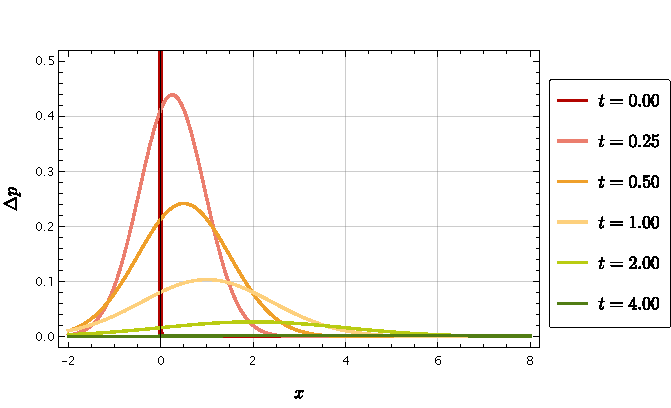
\includegraphics[scale=0.95]{Mathematica/output/DeltPExp.pdf}
\end{Figure}
通过\xref{fig:非平衡载流子的光脉冲注入}可以形象的看出,光脉冲注入中的“漂移--扩散--复合”过程
\begin{itemize}
    \item 漂移使波包的均值增大,表现为波包整体沿电场方向运动,即载流子整体随电场运动。
    \item 扩散使波包的方差增大,表现为波包逐渐变宽变平坦,即载流子向两端浓度低处散开。
    \item 复合使波包的曲线下面积减小,即载流子的总量不断减小。
\end{itemize}

通过光脉冲的例子,现在应该能直观理解“漂移--扩散--复合”是如何共同影响载流子行为了。

